%\documentclass[a4paper,11pt,final]{article}
% Pour une impression recto verso, utilisez plutôt ce documentclass :
\documentclass[a4paper,11pt,twoside,final]{article}

\usepackage[english,francais]{babel}
\usepackage[utf8]{inputenc}
\usepackage[T1]{fontenc}
\usepackage[pdftex]{graphicx}
\usepackage{setspace}
\usepackage{hyperref}
\usepackage[french]{varioref}

\usepackage{fancyvrb}
\usepackage{xcolor}
\usepackage{verbatim}


\newcommand{\reporttitle}{Résolveur de sudoku}     % Titre
\newcommand{\reportauthor}{Loïc Frétard} % Auteur
\newcommand{\reportsubject}{Projet d'application informatique} % Sujet
\newcommand{\HRule}{\rule{\linewidth}{0.5mm}}
\setlength{\parskip}{1ex} % Espace entre les paragraphes

\hypersetup{
    pdftitle={\reporttitle},%
    pdfauthor={\reportauthor},%
    pdfsubject={\reportsubject},%
    pdfkeywords={projet} {application} {informatique} {langage} {java} {algorithmique} {informatique} 
}

\hypersetup{                    % parametrage des hyperliens
    colorlinks=true,                % colorise les liens
    breaklinks=true,                % permet les retours à la ligne pour les liens trop longs
    urlcolor= blue,                 % couleur des hyperliens
    linkcolor= blue,                % couleur des liens internes aux documents (index, figures, tableaux, equations,...)
    citecolor= green                % couleur des liens vers les references bibliographiques
}

\begin{document}
  % Inspiré de http://en.wikibooks.org/wiki/LaTeX/Title_Creation

\begin{titlepage}

\begin{center}

\begin{minipage}[t]{0.48\textwidth}
  \begin{flushleft}
    
\includegraphics [width=30mm]{images/logo-univ.jpg} \\[0.5cm]
    \begin{spacing}{1.5}
      \textsc{L3 Informatique}
    \end{spacing}
  \end{flushleft}
\end{minipage}
\begin{minipage}[t]{0.48\textwidth}
  \begin{flushright}
    %
\includegraphics [width=30mm]{images/logo-societe.jpg} \\[0.5cm]
    %\textsc{\LARGE Entreprise}
    \today
  \end{flushright}
\end{minipage} \\[1.5cm]

\textsc{\Large \reportsubject}\\[0.8cm]
\HRule \\[0.4cm]
{\huge \bfseries \reporttitle \\ Rapport}\\[0.8cm]
\HRule \\[1.5cm]

\parskip=200pt

\begin{minipage}[t]{0.3\textwidth}
  \begin{flushleft} \large
    \emph{Auteurs :}\\
    \reportauthor \\ 
    HARDOUIN Paul \\ 
    BOUCHER Laëtitia \\ 
    BRUN Florian
  \end{flushleft}
\end{minipage}
\begin{minipage}[t]{0.6\textwidth}
  \begin{flushright} \large
    \emph{Responsable :} \\
    M.~ \textsc{Guesnet} \\
  \end{flushright}
\end{minipage}

\vfill

\end{center}

\end{titlepage}

  \tableofcontents % Table des matières
  \sloppy          % Justification moins stricte : des mots ne dépasseront pas des paragraphes
  % \section*{Remerciements}
\addcontentsline{toc}{section}{Remerciements}

Je tiens à remercier \LaTeX{} et les tutoriels sur internet et notamment \url{http://www.ukonline.be/programmation/latex/tutoriel/index.php}.

Bla bla bla bla bla.

  \section{Vocabulaire utilisé}
Cette section a pour but de répertorier 
les différents mots de vocabulaire que nous emploierons dans la suite.\\
\\
Pour la partie code, nous utiliserons les équivalents 
de ces mots en anglais, ils seront noté ci-dessous entre parenthèses.

\begin{itemize}
 \item Sudoku : terme désignant le jeu en lui-même. \\
 
 \item Grille (grid): il s'agit de l'ensemble des régions et des cellules. \\
 
 \item Région (area) : ensemble contenant des cellules. La région est une unité du Sudoku, qui doit obligatoirement contenir une fois chaque 
  symbole, mais une fois seulement. \\
 
 \item Cellule (cell): ensemble pouvant contenir des candidats ou une valeur. \\
 
 \item Heuristiques : termes désignant les règles 
 dont nous nous servirons pour créer nos algorithmes afin de résoudre une grille de sudoku. \\ 
  
 \item Ligne (row) :
 la ligne est une unité du Sudoku, qui doit obligatoirement contenir une fois chaque  
 symbole, mais une fois seulement. \\
 
 \item Colonne (column) :
  la colonne est une unité du Sudoku, qui doit obligatoirement contenir une fois chaque 
  symbole, mais une fois seulement. \\
  
  \item Unité (unit) :
  nous appelons "unités" les diverses parties de la grille de Sudoku: lignes, colonnes, 
  et régions qui présentent des caractéristiques identiques en nombre de cases, 
  de symboles et de règlements. \\
  
  Il y a 27 unités dans une grille standard de Sudoku.
  Diverses méthodes expliquées dans ce guide, s'appliquent indifféremment à toutes les 
  unités d'une grille, alors que d'autres pas. C'est à chaque fois précisé. \\

  \item Symbole (Symbol) :
  vous devez remplir chaque unité du Sudoku avec 9 symboles différents.  \\
 
  Dans une grille standard de Sudoku, on utilise les chiffres 1 2 3 4 5 6 7 8 et 9. 
  Il est possible de trouver des grilles de Sudoku à remplir avec d'autres symboles.  \\

  \item Case (cell) :
  chaque unité de la grille standard de Sudoku contient 9 cases, et chaque case un seul 
  symbole. Il y a 81 cases dans une grille standard. \\

  \item Candidat (candidate) :
  les candidats sont les diverses possibilités de symboles pour une case donnée. 
  Le principe du jeu est de réduire les nombres de candidats pour obtenir le symbole 
  final à faire figurer dans la case.\\
  
  \item Valeur (Value) : 
  une valeur est représentée par un unique symbole pour une case donnée.
  L'objectif étant de fixer une valeur dans chaque case et de trouver les bonnes valeurs.
  
\end{itemize}

\section{Fonctionnalités}

\subsection{Fonctionnalités obligatoires}

\begin{enumerate}
  
  \item Fichier de chargement pour une nouvelle grille :
  l'utilisateur peut demander le chargement d'une grille afin 
  de pouvoir effectuer l'une de deux actions suivantes : 
  la compléter ou la créer afin d'avoir une nouvelle grille. \\
  
  \item Sauvegarde/chargement d’une partie :
  afin de procéder à une sauvegarde, l'utilisateur peut enregistrer la grille actuelle 
  dans un fichier et peut la récupérer ensuite grâce à une option de chargement. \\
  
  \item Réinitialisation de la grille :
  option permettant de remettre la grille de sudoku telle qu'elle était à son chargement. \\
  
  \item Modification d’une cellule :
  une cellule devra être modifiable afin de pouvoir ajouter/retirer des candidats. \\
  
  \item Valeur définitive :
  dans une cellule, on pourra fixer une valeur définitive qui ne sera plus modifiable par la suite. \\
  
  \item Élimination des possibilités pour la valeur sur la ligne, colonne et
  région sur lesquels se trouve la cellule :
  on pourra éliminer plusieurs possibilités d'une cellule par rapport à une région. \\
  
  \item Possibilité : valeur supposée valide d'une cellule dans l'attente de la faire passer en valeur définitive. \\
  
  \item Effacement : permet d'effacer une cellule, de la remettre à zéro. \\
  
  \item Demander l’aide : bouton permettant à l'utilisateur de bénéficier d'une aide 
  afin de résoudre la grille en donnant des indications permettant de ne pas rester bloqué. \\
  
  \item Expliquer la règle : explication d'une règle de résolution. \\
  
  \item Appliquer la règle : permet d'utiliser la règle choisie. \\
  
  \item Résoudre la grille pas à pas : système permettant une résolution 
  de grille de manière pas à pas, c'est-à-dire en résolvant cellule après cellule en appliquant 
  différents algorithmes nécéssitant l'utilisation de règles qui seront communiquées à l'utilisateur. \\
  
  \item Résoudre complètement : solution complète de la grille de sudoku. \\
  
  \item Si la grille ne peut pas être résolue : proposer une réinitialisation 
  avant résolution en indiquant que la grille est irrésolvable. \\
  
  \item Classement par difficultés : grille classée en fonction 
  des heuristiques nécessaires permettant d'évaluer un système de niveaux. \\
  
  \item Annuler : permet de défaire la dernière action action réalisée sur la grille.\\
  
  \item Refaire : permet de défaire l'action annulé. \\

  \item Raccourcis clavier : gestion des appuis simultanés de touches du clavier 
  générant des possibilités inscrites dans le menu tel les sauvegardes/chargements 
  de nouvelles grilles, l'annulation/réactivation d'une action etc.  \\  
  
  \item Demande d’aide : système permettant à l'utilisateur 
  de bénéficier d'une aide en cas de problème. \\

  \item Tutoriel : quelques explications pour tous ceux qui désirent (ré)apprendre 
  à résoudre un sudoku, quelles sont les règles, comment cela fonctionne etc.\\ 
  
  \item Guide : quelques explications sur l'utilisation de l'application 
  (gestion des boutons, comment jouer etc.).\\
 
  \item Masquer la grille pendant la pause : lorsque l'utilisateur appuyera sur le bouton pause, 
  ce dernier verrouillera la session de jeu et ainsi, 
  il ne sera plus possible de jouer tant que l'utilisateur 
  n'aura pas repris le jeu en appuyant sur le bouton reprendre. \\
\end{enumerate}
 
\subsection{Fonctionnalités facultatives}

\begin{enumerate}
  \item Prise en charge de grilles de dimensions variables : 
  l'utilisateur peut demander à avoir une grille de n cases, ainsi,
  si n vaut 2, l'utilisateur pourra utiliser une grille de deux cases sur deux, 
  offrant une grille de 4 cases au total.   \\

 \item Chronomètre : système permettant à l'utilisateur de connaître 
 le temps qu'il a mis à résoudre une grille.  \\
 
 \item Éditeur/générateur : possibilités pour l'utilisateur 
 de créer ses propres grilles selon des niveaux de difficultés. \\
 
 \item Samourai : système de jeu impliquant 5 grilles de sudoku formant une grille géante 
 disposé de telle sorte à ce qu'une grille centrale soit partagé 
 par les 4 autres grilles disposés au coin de cette dernière.  \\
\end{enumerate}

\section{Implantation}
Pour implanter notre sudoku, nous avons choisi de fonctionner selon le modèle MVC, 
c'est-à-dire le système Modèle-Vue-Contrôleur. Afin de visualiser notre organisation, 
des diagrammes ont été réalisés et sont disponibles en annexe 
(annexe 18 : diagramme model,
annexe 19 : diagramme history,
annexe 20 : diagramme heuristic).

\subsection{SudokuModel}
Le sudoku possède deux grilles(GridModel) : celle du joueur et la solution. 
Le sudoku est aussi composé d'un historique.\\
La grille solution est générée par application des heuristiques à l’aide 
d’un gestionnaire d’heuristiques (RuleManager). La grille
joueur est le résultat des interactions du joueur(ajouter/supprimer un candidat 
ou sélectionner/désélectionner une valeur). \\
L’historique répertorie les actions du joueur avec possibilité d’annuler ses actions.\\ 
Le joueur a gagné quand sa grille est finie, sans conflits de nombres 
(deux 6 sur la même ligne par exemple).\\
La partie est finie quand le joueur a rempli toutes les cases de sa grille d’une valeur. 
À tout moment le joueur peut demander de l’aide ou demander un indice (exécution d’une
heuristique). On peut sauvegarder ou enregistrer sa partie ou encore générer une grille
à partir d’un fichier texte (sur la première ligne doit se trouver la hauteur
et la largeur de la grille puis sur les lignes qui suivent les valeurs des cases
fixes du sudoku). Le joueur peut à tout moment réinitialiser sa partie, c’est
à dire, mettre sa grille comme elle était avant toute interaction de sa part,
seules les valeurs des cases fixes restent.

\subsection{GridModel}
Une grille possède une taille n (hauteur x largeur) fixe, inchangeable donnée en paramètre lors de l'initialisation et
un tableau à double entrée (lignes, colonnes) de cellules (ModelCell).
La grille connait son nombre de valeurs/candidats possibles.
Une coordonnée (ICoord) représente une des cases du tableau : elle commence de 0 et va jusqu'à n - 1.
Elle peut donner la cellule par rapport à une coordonnée et inversement, mais aussi un ensemble de cellules d'une
unité (colonne, ligne, région) d'une cellule en lui donnant soit sa coordonnée soit elle-même en paramètre.
La grille possède un détecteur de validation de coordonnée pour vérifier que la coordonnée est toujours dans le tableau. 
De même que SudokuModel, on peut ajouter/supprimer un candidat de la grille ou ajouter/supprimer (si ce n'est pas une 
case fixe) une valeur.

\subsection{CellModel}
Une cellule possède un tableau de candidat.
Une cellule peut être soit modifiable, c'est-à-dire qu'on peut modifier sa valeur, ou soit fixe, immuable : 
ce sont les cases du départ de la grille. 
Comme la grille, elle connait son nombre de valeurs/candidats possibles qui est donné en paramètre.
La cellule a soit une valeur, soit une liste de candidats possibles. 
On peut ajouter/supprimer un candidat de la cellule ou ajouter/supprimer (si ce 
n'est pas une case fixe) une valeur. On peut aussi demander à tout moment sa valeur, si une valeur est un candidat
potentiel pour cette cellule ou même inverser ces candidats (si un nombre était un candidat potentiel ce n'est plus
le cas et inversement).

\subsection{Command}
Une commande est un objet capable de modifier une grille selon certains critères (ajout/suppression candidat, ajout/suppression valeur).
AbstractCommand est la classe fournissant un mécanisme général pour les commandes, elle est la super classe de 
AddValue (ajoute une valeur à la cellule), AddCandidate (ajoute un candidat à la cellule),
RemoveValue (supprime une valeur à la cellule), RemoveCandidate (supprime un candidat à la cellule).

\subsection{History}
L'historique est une sorte de pile chronologique bornée. On peut toujours ajouter des éléments (Command) à un historique : lorsque l'historique est plein, rajouter un nouvel élément fait disparaître le plus ancien. On peut avancer et 
reculer le curseur repérant l'élément courant à loisir dans l'historique, mais si le curseur n'est pas sur l'élément le 
plus récent, ajouter un élément dans l'historique à cet instant fait disparaître les éléments postérieurs au curseur.

\subsection{RuleManager}
Deux comportements possibles existent pour une heuristique : soit on trouve la valeur à mettre dans la case 
(exemple : seul candidat), soit on peut supprimer des candidats dans les cases de la grille (exemple : jumeaux et triplet)
ce qui réduit les possibiltés de valeurs à chaque boucle d'heuristique.
Le gestionnaire va parcourir les heuristiques de la plus simple à la plus complexe (qui sont classées dans une classe énumerative Rule où
chaque algorithme de résolution est associé à une unique heuristique) pour trouver celle qui apporte une solution.
Le gestionnaire peut demander à tout moment la description ou l'execution de la dernière solution trouvée.
L'heuristique choisie est un rapport (Report).

\subsection{Report}
Le rapport répertorie les cellules qui sont en lien avec l'action (suppression ou ajout de candidats/valeur) ou les cellules
qui ont aidé à ce raisonnement. Elle possède une description qui lui est propre en rapport avec l'heuristique et 
une exécution des commandes (suppression candidats ou ajout valeur).

\section{Heuristiques implantées}
\subsection{Un seul candidat : (only candidate)}
C'est l'heuristique la plus simple. Si une case ne contient qu'un candidat c'est que ce candidat est la valeur 
finale de la case obligatoirement.\\
\\

Exemple : \\
On peut voir ici que sur la troisième ligne et la sixième colonne se trouve le candidat 4.
Comme étant le seul candidat dans cette case, de ce fait, on peut le sélectionner comme valeur.\\

\begin{figure}[ht]
  \caption{\label{annexe1} seul candidat}
  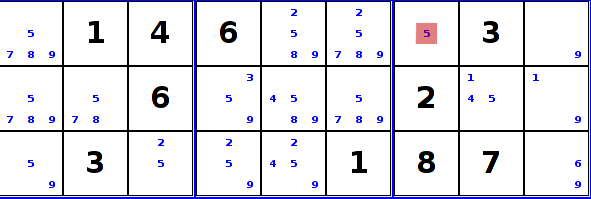
\includegraphics [width=80mm]{images/only-candidate.png} \\[0.5cm]
\end{figure}

\newpage

\subsection{Un candidat unique : (one candidate)}
Prenons maintenant une ligne complète. Dans les cases vides, nous avons noté la liste des candidats potentiels. 
Chaque chiffre de 1 à 9 devant obligatoirement se trouver sur la ligne de façon unique, si dans les candidats 
de toutes les cases de la ligne, un candidat n'apparait qu'une seule fois, alors c'est qu'il doit effectivement 
être placé dans cette case.
Il est possible d'utiliser cette méthode dans toutes les unités de la grille (lignes, colonnes, régions).

Exemple :
On peut voir ici que sur la première ligne, deuxième colonne, il y a un seul candidat 
dans la case. Donc il n'y a qu'une solution : 5.\\

\begin{figure}[ht]
  \caption{\label{annexe2} candidat unique}
  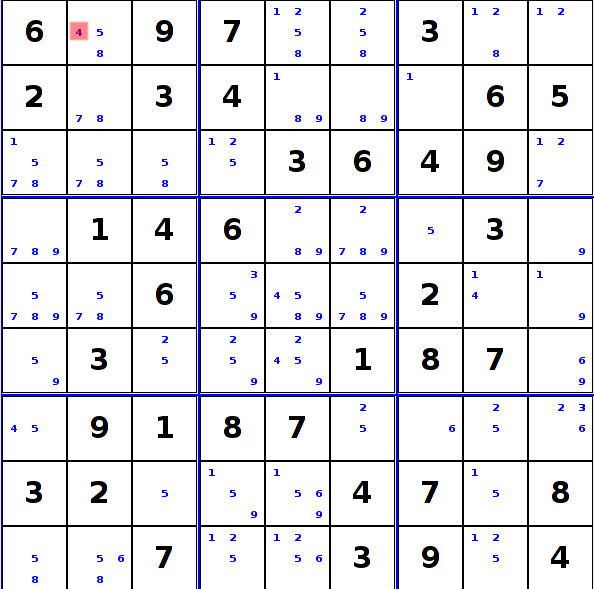
\includegraphics [width=100mm]{images/one-candidate.png} \\[0.5cm]
\end{figure}


\subsection{Des jumeaux/triplés : (pair/triplet)}
Il n'est pas toujours possible de découvrir dès le début l'emplacement final et définitif d'un symbole. 
Cependant il est parfois possible de savoir dans quelle ligne ou colonne il ne se trouve pas, et donc 
d'en déduire dans quelle partie de la région il va finir par se trouver.
Quand une unité contient deux cases avec une même paire de candidats (et eux seuls) alors ces candidats 
ne peuvent se trouver dans une autre case de l'unité. \\
\\
Si ce n'est pas suffisant pour pouvoir le placer immédiatement. C'est cependant très utile pour 
supprimer les candidats de cette ligne.
Les triplés fonctionnent exactement sur le même principe, mais avec 3 symboles libres dans la même 
ligne ou colonne de la région.\\
\\
Il est possible d'utiliser cette méthode dans toutes les régions alignées (horizontalement ou verticalement) 
et dans toutes les lignes ou colonnes.
Si à l’intérieur d’un bloc, un chiffre n’est possible que dans une ligne/colonne, alors
nous pouvons en déduire que ce chiffre ne peut pas être présent dans les cases de cette
ligne/colonne n’appartenant pas au bloc.\\
\\
Exemple :\\
On peut voir ici que sur la région centrale, les 1 sont uniquement présents 
et alignés sur la verticale.
Si bien qu'on peut en déduire qu'un des deux 1 est la solution, 
donc on peut supprimer les autres de la colonne.\\

\begin{figure}[ht]
  \caption{\label{annexe3} jumeaux, triplés}
  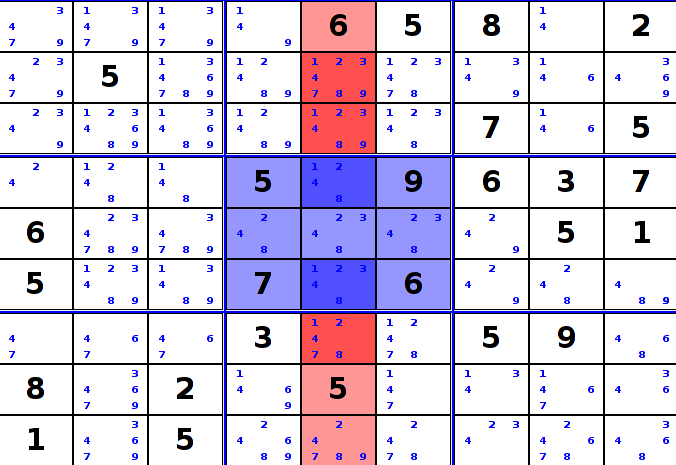
\includegraphics [width=100mm]{images/PairTriplet.png} \\[0.5cm]
\end{figure}

\newpage

\subsection{Interactions entre régions}
Si à l’interieur d’une ligne/colonne, un chiffre n’est possible que dans un bloc, alors
nous pouvons en déduire que ce chiffre ne peut pas être présent dans les autres cases de
ce bloc.\\
\\

Exemple :\\
Dans cet exemple, on peut constater que dans R7 et R9, le 8 n'est pas présent sur L8. 
On peut donc supprimer les 8 dans la R8 à l'exception de ceux sur L8.

\begin{figure}[ht]
  \caption{\label{annexe4} Interactions entre régions}
  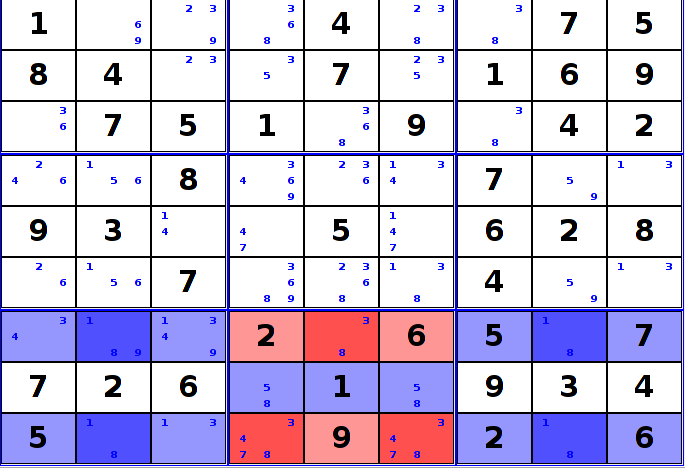
\includegraphics [width=100mm]{images/InteractionBetweenSector.png} \\[0.5cm]
\end{figure}

\subsection{Candidats identiques}
Cette méthode ne donne pas la possibilité de répondre à la question du choix,
mais donne la possibilité de supprimer des candidats indésirables.
Car, en effet, si deux cases ne contiennent que deux fois les mêmes candidats
On peut être certain que ces deux candidats vont finalement terminer dans l'une
et dans l'autre. Et donc supprimer ces candidats des autres cases.\\
\\
Cette méthode s'applique dans les cas suivants:\\
- avec 2 candidats dans 2 cases\\
- avec 3 candidats dans 3 cases\\
- avec 4 candidats dans 4 cases\\
...\\
- avec N candidats dans N cases\\
\\
Il est possible d'utiliser cette méthode dans toutes les unités de la grille.

\subsection{X-Wing}
Le nom X-Wing (ou aile en X) provient de la figure tracée par cette méthode. \\
En effet le principe est basé sur le choix à faire dans l'emplacement d'une valeur. \\
En effet si une valeur est placée dans un coin, la même valeur ne pourra être placée que dans le coin opposé, 
ce qui trace les diagonales des 2 possibilités.\\
\\
Il est nécessaire de trouver 2 unités (lignes, colonnes ou régions) dans lesquelles on ne trouve que 2 candidats pour une même valeur. Et qu'en plus on retrouve cette correspondance dans 2 unités du même type, reliées par des unités communes aux unités de base. Pour pouvoir supprimer les autres candidats des unités communes.
\\
Cette méthode s'applique dans les cas suivants, avec 2 candidats:\\
- dans 2 colonnes, en supprimant les candidats dans 2 lignes\\
- dans 2 colonnes, en supprimant les candidats dans 2 régions\\
- dans 2 lignes, en supprimant les candidats dans 2 colonnes\\
- dans 2 lignes, en supprimant les candidats dans 2 régions\\
- dans 2 régions, en supprimant les candidats dans 2 lignes\\
- dans 2 régions, en supprimant les candidats dans 2 colonnes\\
\\
Il est possible d'utiliser cette méthode dans toutes les unités de la grille (régions, lignes, colonnes).
\\

Exemple :\\
Dans cet exemple, il n'est possible de trouver le candidat 5 
qu'à deux emplacements des lignes L2 et L8.\\ 
De plus, ces candidats font partie des colonnes communes C5 et C7.\\ 
Il est donc possible de supprimer tous les autres candidats 5 de ces 2 colonnes. 

\begin{figure}[ht]
  \caption{\label{annexe5} XWing}
  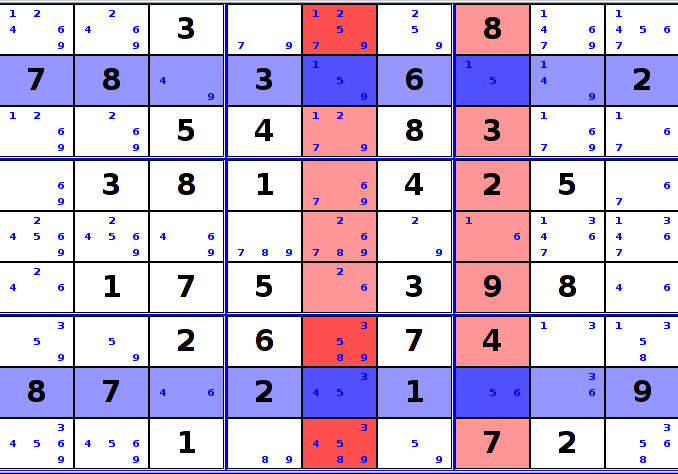
\includegraphics [width=100mm]{images/XWing.png} \\[0.5cm]
\end{figure}

\newpage

\subsection{Groupes isolés}
Si 3 candidats se retrouvent seuls dans 3 cases, il est possible de savoir qu'ils finiront bien dans ces 3 cases. 
Même si les 3 candidats ne sont pas présents dans les 3 cases et donc supprimer ces candidats des autres cases.
\\
Cette méthode s'applique dans les cas suivants:\\
- avec 2 candidats dans 2 cases\\
- avec 3 candidats dans 3 cases\\
- avec 4 candidats dans 4 cases\\
...\\
- avec N candidats dans N cases\\

Il est possible d'utiliser cette méthode dans toutes les unités de la grille (régions, lignes, colonnes).

\subsection{Groupes mélangés}
Cette méthode ressemble beaucoup à celle expliquée sous "Groupes isolés". 
Mais son application n'est pas la même car elle ne concerne que les cases qui contiennent les candidats, 
et pas les autres.\\
\\

Si on ne retrouve 3 candidats, que dans 3 cases, on est certain qu'ils vont terminer dans ces 3 cases.\\ 
Il est donc possible de supprimer les autres candidats de ces dernières.\\
\\
Cette méthode s'applique dans les cas suivants:\\
- avec 2 candidats dans 2 cases de X candidats\\
- avec 3 candidats dans 3 cases de X candidats\\
- avec 4 candidats dans 4 cases de X candidats\\
...\\
- avec N candidats dans N cases de X candidats\\
\\
La méthode des "Groupes isolés" permettait de supprimer les candidats des autres cases, 
alors que celle-ci donne la possibilité de supprimer les autres candidats dans les mêmes cases.\\
\\
De plus, avec cette méthode, il est nécessaire de ne trouver les candidats concernés que dans 
les cases utilisées (alors que c'est justement l'inverse qui est utile dans l'autre méthode).\\
Il est possible d'utiliser cette méthode dans toutes les unités de la grille (régions, lignes, colonnes).





\end{document}

